\section{VQA and QNN}
\begin{itemize}
    \item Basic concepts: \textbf{Cost function, ansatz, gradients, optimizers}
    \item Global and local cost function
    \item Some illustration?
\end{itemize}

Hybrid techniques involving Quantum circuits and Classical optimisers have been proposed to overcome the restrictions of Noisy Intermediate-Scale Quantum (NISQ) \cite{brooksQuantumSupremacyHunt2019} devices. 
Those constraints are the absence of fault-tolerant design, the limitation of qubit number per processor, and executable circuit depth. 
Moreover, quantum gates are static by design, which means every new data input to a quantum algorithm will produce a different quantum circuit.

Quantum circuits with trainable parameters can be created using Variational Quantum Algorithms (VQAs) \cite{cerezo2021variational}, which act as reusable circuit templates for quantum computers.
On the other hand, the classical optimiser perceives variational circuits as a black box that yields outputs from inputs and the trainable parameter.

Consider a simple problem that we want to solve using VQA, given access to the training data.
The first step is to define a \textit{cost function} $C$ to search for a solution, and we aim to minimise this cost function during the training process.
Then, we develop an \textit{ansatz}; this is the unitary operation that depends on a set of parameters $\theta$. We aim to train this ansatz to optimise $\theta$ such that the cost function $C$ reaches its minimum, thus satisfying:
\begin{equation}
    \theta^* = \underset{\theta}{\arg \min} C(\theta)
    \label{optimize theta with ansatz}
\end{equation}

In short, the cost function $C(\theta)$ is calculated using the Quantum computer, while the classical optimisers train the parameter $\theta$. The Figure \ref{VQA diagram} elaborates on the VQA architecture and process in more detail.

\begin{figure}
    \centering
    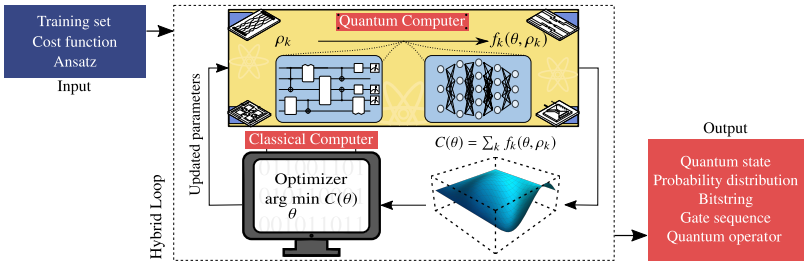
\includegraphics[width=\textwidth]{LiteratureReview/Appendices/vqadiagram.png}
    \caption{
    An illustrative diagram of VQA. The algorithm receives: 
    A cost function $C(\theta)$ for $\theta$ is a set of parameters that encodes the solution; 
    An ansatz that receives trainable parameter $\theta$ in the hybrid loop to solve the task;
    A set of training data $\{\rho_k\}$.
    We use the quantum computer to calculate the cost for each iteration, then pass this information to the classical computer that uses an optimiser to navigate the cost landscape $C(\theta)$ and solve the problem in Eq. (\ref{optimize theta with ansatz}).
    The output of VQA is an estimate of the solution to the problem, which can take forms as in the red box.
    Figure from ref \cite{cerezo2021variational}.
    }
    \label{VQA diagram}
\end{figure}

\subsection{The Cost Function}
Encoding the problem into a cost function is the first step to solving a problem using VQA.
This cost function is the same  compared to classical machine learning. It maps the values of the trainable parameters $\theta$ into real numbers.
For a function $f$ that receives input states $\{\rho_k\}$, observables $\{O_k\}$, and a parameterized circuit $U(\theta)$, the cost is expressed as:
\begin{equation}
    C(\theta) = f(\{\rho_k\}, \{O_k\}, U(\theta)) \;,
\end{equation}
or this form with a set of functions $\{ f_k \}$:
\begin{equation}
    C(\theta) = \sum_k f_k \left(\Tr[ O_k U(\theta) \rho_k U^\dagger(\theta) ]\right) \;,
    \label{Cost function}
\end{equation}

There are some criteria in the construction of a cost function: 
(1) The cost function must be 'faithful' and 'operational meaningful', such that the minimum of $C(\theta)$ should correspond to the solution of the problem, and the lower cost function indicate a better solution in general;
(2) Cost function must be 'efficiently estimated' by measurement on a quantum computer and classical post-processing;
(3) The cost must be 'trainable', such that the parameters $\theta$ should be efficiently optimised.

\subsection{The Ansatzes}
\begin{figure} 
    \centerline{
        \Qcircuit @C=1em @R=0em {
        & \multigate{2}{U_1(\theta_1)}    & \multigate{2}{U_2(\theta_2)}    & \qw &        & & \multigate{2}{U_L(\theta_L)}   & \qw\\
        & \ghost{U_1(\theta_1)}           & \ghost{U_2(\theta_2)}           & \qw & \cdots & & \ghost{U_L(\theta_L)}          & \qw\\
        & \ghost{U_1(\theta_1)}           & \ghost{U_2(\theta_2)}           & \qw &        & & \ghost{U_L(\theta_L)}          & \qw
        \gategroup{1}{2}{3}{7}{.6em}{--}
        }
    }
    \centerline{$U(\theta)$}
    \centerline{
        \Qcircuit @C=1em @R=0em{
        & \multigate{1}{}   & \ctrl{2}  & \gate{}           & \qw \\
        & \ghost{}          & \qw       & \multigate{1}{}   & \qw \\
        & \gate{}           & \targ     & \ghost{}          & \qw
        \gategroup{1}{2}{3}{4}{.6em}{--}
        }
    }
    \centerline{$U_l(\theta_l)$}
    \caption{
        A diagram of an ansatz.
        The unitary $U(\theta)$ receives parameters $\theta$ is expressed by $L$ layers of unitaries $U_l(\theta_l)$ for $l$ is the layer indices.
        Each $U_l(\theta_l)$ is a circuit of parameterized or unparameterized gates.
    }\label{Ansatz diagram}
\end{figure}

The 'ansatze' is the parameterised circuit, parameterised unitary, or variational circuit.
In general, the parameters $\theta$ are determined by the ansatz form and thus can be trained to minimise the cost.
The ansatz structure can be defined based on the problem (called 'problem-inspired ansatzes) or a generic structure (called 'problem agnostic') that can be used without any relevant information available.
The cost function in Eq. (\ref{Cost function}) encodes the parameters $\theta$ in a unitary $U(\theta)$ and applies to the input states of the circuit. The figure \ref{Ansatz diagram} shows that $U(\theta)$ can be expressed as a product of $L$ continuously unitaries:
\begin{equation}
    U(\theta) = U_L(\theta_L) \cdots U_2(\theta_2) U_1(\theta_1)\;,
\end{equation}
with each layer:
\begin{equation}
    U_l(\theta_l) = \prod_m e^{-i\theta_m H_m} W_m
\end{equation}
for unparamaterized unitary $W_m$, Hermitian Operator $H_m$, and $\theta_l$ is the $l$-th element of $\theta$

\subsection{The Gradients}
After defining the cost function and ansatz, we train the parameter $\theta$ to solve the problem in Eq. (\ref{optimize theta with ansatz}).
The cost function gradient helps the optimiser to find the global minima. 
Consider the cost function in Eq. (\ref{Cost function}), for a parameterized unitary $e^{i \theta_l \sigma}$, let $\theta_l$ be the $l$-th element of $\theta$, $\sigma_l$ is a Pauli operator. 
We can evaluate the gradient with the Parameter-shift rule:
\begin{equation}
    \frac{\partial C}{\partial\theta_l}
    = \sum_k \frac{1}{2 \sin{\alpha}} 
    \left( 
        \Tr[O_k U^\dagger(\theta_+) \rho_k U(\theta_+)] 
        - \Tr[O_k U^\dagger(\theta_-) \rho_k U(\theta_-)]
    \right) \;,
    \label{Parameter-shift rules}
\end{equation}
with $\theta_{\pm} = \theta \pm \alpha e_l$, $\alpha \in \mathbb{R}$ and $e_l$ is a vector such that its $l$-th position have the value of 1, or else 0.

Essentially, we can shift the $l$-th parameter by some amount $\alpha$, and Eq. (\ref{Parameter-shift rules}) will evaluate the gradient. 


\subsection{The Optimisers}
The accuracy of VQA greatly depends on the optimisation method.
Typically, we can achieve the solution by making successive moves along the gradient's direction.
This optimisation approach is within the scope of Stochastic Gradient Descent (SGD).
One example of SGD is the ADAM optimiser \cite{kingmaAdamMethodStochastic2014}, which can vary the size of the steps taken during optimisation to produce more efficient and precise results compared to the basic SGD.


\subsection{About QNN}
VQA is also the most widely used method for developing Quantum Neural Network (QNN) circuits. 
As a result, QNN inevitably inherited some of VQA's flaws.
Many Quantum Machine Learning models suffer from the unsolvability Barren Plateaus \cite{zhaoReviewQuantumNeural2021} that prevent the growth of circuit depth and lead the trainable parameters to a dead end.
When training a QNN framework with a large number of qubits, this phenomenon occurs; the objective function becomes flat, making it nearly impossible to estimate the gradient, \cite{mccleanBarrenPlateausQuantum2018, zhaoAnalyzingBarrenPlateau2021} causing inefficiency in circuit training. We will discuss this matter in later sections.

Some architectures of QNN has been proposed are: 
Quantum Tensor Neural Network (QTNN) \cite{hugginsQuantumMachineLearning2019} achieved a balance of computational efficiency and expressive power. 
The tensor network can reduce the required qubits to process high-dimensional data with powerful optimisation algorithms.
Quantum Recurrent Neural Network (QRNN) is constructed as a parameterised circuit \cite{takakiLearningTemporalData2021}, with some qubits being initialised and measured at each step while others memorise the past data.
The NISQ processors are also capable of delivering some other QNN models such as: 
Quantum Boltzmann Machine \cite{shinguBoltzmannMachineLearning2021, zoufalVariationalQuantumBoltzmann2021}, 
Quantum Perceptron \cite{kristensenArtificialSpikingQuantum2021}, 
Quantum Generative Adversarial Network \cite{dallaire-demersQuantumGenerativeAdversarial2018, lloydQuantumGenerativeAdversarial2018}. Studies have shown that QNN performance and trainability can be significantly higher compared to its classical counterpart on today's hardware \cite{abbasPowerQuantumNeural2021, colesSeekingQuantumAdvantage2021}, and has several applications, for example, breast cancer prediction \cite{liModelAlgorithmQuantuminspired2014}, or image processing \cite{matsuiQubitNeuralNetwork2009}.

It is noticeable that Quantum Convolutional Neural Network (QCNN) does not exhibit Barren Plateaus \cite{pesahAbsenceBarrenPlateaus2021}.
Thus, trainability is guaranteed for QCNN under random initialisation.